\hypertarget{mvt_8f}{
\section{mvt.f File Reference}
\label{mvt_8f}\index{mvt.f@{mvt.f}}
}
\subsection*{Functions}
\begin{CompactItemize}
\item 
subroutine \hyperlink{mvt_8f_4b51e2fd2b5378c70a36771ac4cfed04}{MVTDST} (N, NU, LOWER, UPPER, INFIN, CORREL, DELTA, MAXPTS, ABSEPS, RELEPS, ERROR, VALUE, INFORM)
\item 
subroutine \hyperlink{mvt_8f_1e3a3eb63d17fe37f686fc1f571beccc}{MVSUBR} (N, W, NF, F)
\item 
subroutine \hyperlink{mvt_8f_cb964c59585b62348fb9653f052c669e}{MVSPCL} (ND, NU, A, B, DL, COV, INFI, SNU, VL, ER, INFORM)
\item 
subroutine \hyperlink{mvt_8f_7319671edcfbb7bd0e50690518e644fc}{MVVLSB} (N, W, R, DL, INFI, A, B, COV, Y, DI, EI, ND, VALUE)
\item 
subroutine \hyperlink{mvt_8f_e6a30b16d74f1c585c70de45080c0805}{MVSORT} (N, LOWER, UPPER, DELTA, CORREL, INFIN, Y, PIVOT, ND, A, B, DL, COV, INFI, INFORM)
\item 
DOUBLE PRECISION \hyperlink{mvt_8f_7edd239860c89b5fa9fb100b194fa833}{MVTDNS} (NU, X)
\item 
subroutine \hyperlink{mvt_8f_ae28c99f4b4ff2300cfa96ffa62bf799}{MVLIMS} (A, B, INFIN, LOWER, UPPER)
\item 
subroutine \hyperlink{mvt_8f_2a36c253875e26e22bbb20a386c9a580}{MVSSWP} (X, Y)
\item 
subroutine \hyperlink{mvt_8f_5411cfeafe20ca2bd17c962f8c8c0e84}{MVSWAP} (P, Q, A, B, D, INFIN, N, C)
\item 
DOUBLE PRECISION \hyperlink{mvt_8f_a0072dd6ba4c47d28d78d231b5af9571}{MVPHI} (Z)
\item 
DOUBLE PRECISION \hyperlink{mvt_8f_9ce2ff2aa4833561178c981ac2469470}{MVPHNV} (P)
\item 
DOUBLE PRECISION \hyperlink{mvt_8f_01b86430a337d3d8b91bcf9346d7dd3b}{MVBVN} (LOWER, UPPER, INFIN, CORREL)
\item 
DOUBLE PRECISION \hyperlink{mvt_8f_151b69372f580727b65189d3ba4c08e4}{MVBVU} (SH, SK, R)
\item 
DOUBLE PRECISION \hyperlink{mvt_8f_33d5a1ab44132a99ec34a2a0c899cdcb}{MVSTDT} (NU, T)
\item 
DOUBLE PRECISION \hyperlink{mvt_8f_9d0fae33894aee91124b4f3695494f7e}{MVBVT} (NU, LOWER, UPPER, INFIN, CORREL)
\item 
DOUBLE PRECISION \hyperlink{mvt_8f_597ed59b5410765b8afcc6527c9552e7}{MVBVTC} (NU, L, U, INFIN, RHO)
\item 
double precision \hyperlink{mvt_8f_9194afe3b3514326417468c9e9f43f0e}{mvbvtl} (nu, dh, dk, r)
\item 
DOUBLE PRECISION \hyperlink{mvt_8f_3652f2cb737bf864d78fff1a650ca287}{MVCHNV} (N, P)
\item 
DOUBLE PRECISION \hyperlink{mvt_8f_81b566eaa4178de04b31e15475cde3bf}{MVCHNC} (LKN, N, P, R)
\item 
subroutine \hyperlink{mvt_8f_53a2e447659c04eb0ad551cf58c77d37}{MVKBRV} (NDIM, MINVLS, MAXVLS, NF, FUNSUB, ABSEPS, RELEPS, ABSERR, FINEST, INFORM)
\item 
subroutine \hyperlink{mvt_8f_6b32b1cb4d3243c9ffef2622d8cfa65d}{MVKRSV} (NDIM, KL, VALUES, PRIME, VK, NF, FUNSUB, X, R, PR, FS)
\item 
DOUBLE PRECISION \hyperlink{mvt_8f_1ab822a6524a9096bf2ec00253f890e3}{MVUNI} ()
\end{CompactItemize}


\subsection{Function Documentation}
\hypertarget{mvt_8f_01b86430a337d3d8b91bcf9346d7dd3b}{
\index{mvt.f@{mvt.f}!MVBVN@{MVBVN}}
\index{MVBVN@{MVBVN}!mvt.f@{mvt.f}}
\subsubsection[{MVBVN}]{\setlength{\rightskip}{0pt plus 5cm}DOUBLE PRECISION MVBVN (DOUBLE PRECISION,dimension($\ast$) {\em LOWER}, \/  DOUBLE PRECISION,dimension($\ast$) {\em UPPER}, \/  INTEGER,dimension($\ast$) {\em INFIN}, \/  DOUBLE PRECISION {\em CORREL})}}
\label{mvt_8f_01b86430a337d3d8b91bcf9346d7dd3b}




Definition at line 659 of file mvt.f.

References MVBVU().

Referenced by MVBVT().

Here is the call graph for this function:\nopagebreak
\begin{figure}[H]
\begin{center}
\leavevmode
\includegraphics[width=134pt]{mvt_8f_01b86430a337d3d8b91bcf9346d7dd3b_cgraph}
\end{center}
\end{figure}
\hypertarget{mvt_8f_9d0fae33894aee91124b4f3695494f7e}{
\index{mvt.f@{mvt.f}!MVBVT@{MVBVT}}
\index{MVBVT@{MVBVT}!mvt.f@{mvt.f}}
\subsubsection[{MVBVT}]{\setlength{\rightskip}{0pt plus 5cm}DOUBLE PRECISION MVBVT (INTEGER {\em NU}, \/  DOUBLE PRECISION,dimension($\ast$) {\em LOWER}, \/  DOUBLE PRECISION,dimension($\ast$) {\em UPPER}, \/  INTEGER,dimension($\ast$) {\em INFIN}, \/  DOUBLE PRECISION {\em CORREL})}}
\label{mvt_8f_9d0fae33894aee91124b4f3695494f7e}




Definition at line 858 of file mvt.f.

References MVBVN().

Referenced by MVBVTC(), and MVSPCL().

Here is the call graph for this function:\nopagebreak
\begin{figure}[H]
\begin{center}
\leavevmode
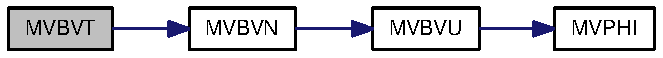
\includegraphics[width=177pt]{mvt_8f_9d0fae33894aee91124b4f3695494f7e_cgraph}
\end{center}
\end{figure}
\hypertarget{mvt_8f_597ed59b5410765b8afcc6527c9552e7}{
\index{mvt.f@{mvt.f}!MVBVTC@{MVBVTC}}
\index{MVBVTC@{MVBVTC}!mvt.f@{mvt.f}}
\subsubsection[{MVBVTC}]{\setlength{\rightskip}{0pt plus 5cm}DOUBLE PRECISION MVBVTC (INTEGER {\em NU}, \/  DOUBLE PRECISION,dimension($\ast$) {\em L}, \/  DOUBLE PRECISION,dimension($\ast$) {\em U}, \/  INTEGER,dimension($\ast$) {\em INFIN}, \/  DOUBLE PRECISION {\em RHO})}}
\label{mvt_8f_597ed59b5410765b8afcc6527c9552e7}




Definition at line 909 of file mvt.f.

References MVBVT().

Here is the call graph for this function:\nopagebreak
\begin{figure}[H]
\begin{center}
\leavevmode
\includegraphics[width=223pt]{mvt_8f_597ed59b5410765b8afcc6527c9552e7_cgraph}
\end{center}
\end{figure}
\hypertarget{mvt_8f_9194afe3b3514326417468c9e9f43f0e}{
\index{mvt.f@{mvt.f}!mvbvtl@{mvbvtl}}
\index{mvbvtl@{mvbvtl}!mvt.f@{mvt.f}}
\subsubsection[{mvbvtl}]{\setlength{\rightskip}{0pt plus 5cm}double precision mvbvtl (integer {\em nu}, \/  double precision {\em dh}, \/  double precision {\em dk}, \/  double precision {\em r})}}
\label{mvt_8f_9194afe3b3514326417468c9e9f43f0e}




Definition at line 962 of file mvt.f.\hypertarget{mvt_8f_151b69372f580727b65189d3ba4c08e4}{
\index{mvt.f@{mvt.f}!MVBVU@{MVBVU}}
\index{MVBVU@{MVBVU}!mvt.f@{mvt.f}}
\subsubsection[{MVBVU}]{\setlength{\rightskip}{0pt plus 5cm}DOUBLE PRECISION MVBVU (DOUBLE PRECISION {\em SH}, \/  DOUBLE PRECISION {\em SK}, \/  DOUBLE PRECISION {\em R})}}
\label{mvt_8f_151b69372f580727b65189d3ba4c08e4}




Definition at line 704 of file mvt.f.

References MVPHI().

Referenced by MVBVN().

Here is the call graph for this function:\nopagebreak
\begin{figure}[H]
\begin{center}
\leavevmode
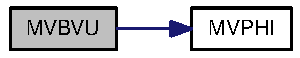
\includegraphics[width=90pt]{mvt_8f_151b69372f580727b65189d3ba4c08e4_cgraph}
\end{center}
\end{figure}
\hypertarget{mvt_8f_81b566eaa4178de04b31e15475cde3bf}{
\index{mvt.f@{mvt.f}!MVCHNC@{MVCHNC}}
\index{MVCHNC@{MVCHNC}!mvt.f@{mvt.f}}
\subsubsection[{MVCHNC}]{\setlength{\rightskip}{0pt plus 5cm}DOUBLE PRECISION MVCHNC (DOUBLE PRECISION {\em LKN}, \/  INTEGER {\em N}, \/  DOUBLE PRECISION {\em P}, \/  DOUBLE PRECISION {\em R})}}
\label{mvt_8f_81b566eaa4178de04b31e15475cde3bf}




Definition at line 1104 of file mvt.f.

References MVPHI().

Referenced by MVCHNV().

Here is the call graph for this function:\nopagebreak
\begin{figure}[H]
\begin{center}
\leavevmode
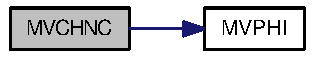
\includegraphics[width=93pt]{mvt_8f_81b566eaa4178de04b31e15475cde3bf_cgraph}
\end{center}
\end{figure}
\hypertarget{mvt_8f_3652f2cb737bf864d78fff1a650ca287}{
\index{mvt.f@{mvt.f}!MVCHNV@{MVCHNV}}
\index{MVCHNV@{MVCHNV}!mvt.f@{mvt.f}}
\subsubsection[{MVCHNV}]{\setlength{\rightskip}{0pt plus 5cm}DOUBLE PRECISION MVCHNV (INTEGER {\em N}, \/  DOUBLE PRECISION {\em P})}}
\label{mvt_8f_3652f2cb737bf864d78fff1a650ca287}




Definition at line 1054 of file mvt.f.

References MVCHNC(), and MVPHNV().

Referenced by MVSUBR().

Here is the call graph for this function:\nopagebreak
\begin{figure}[H]
\begin{center}
\leavevmode
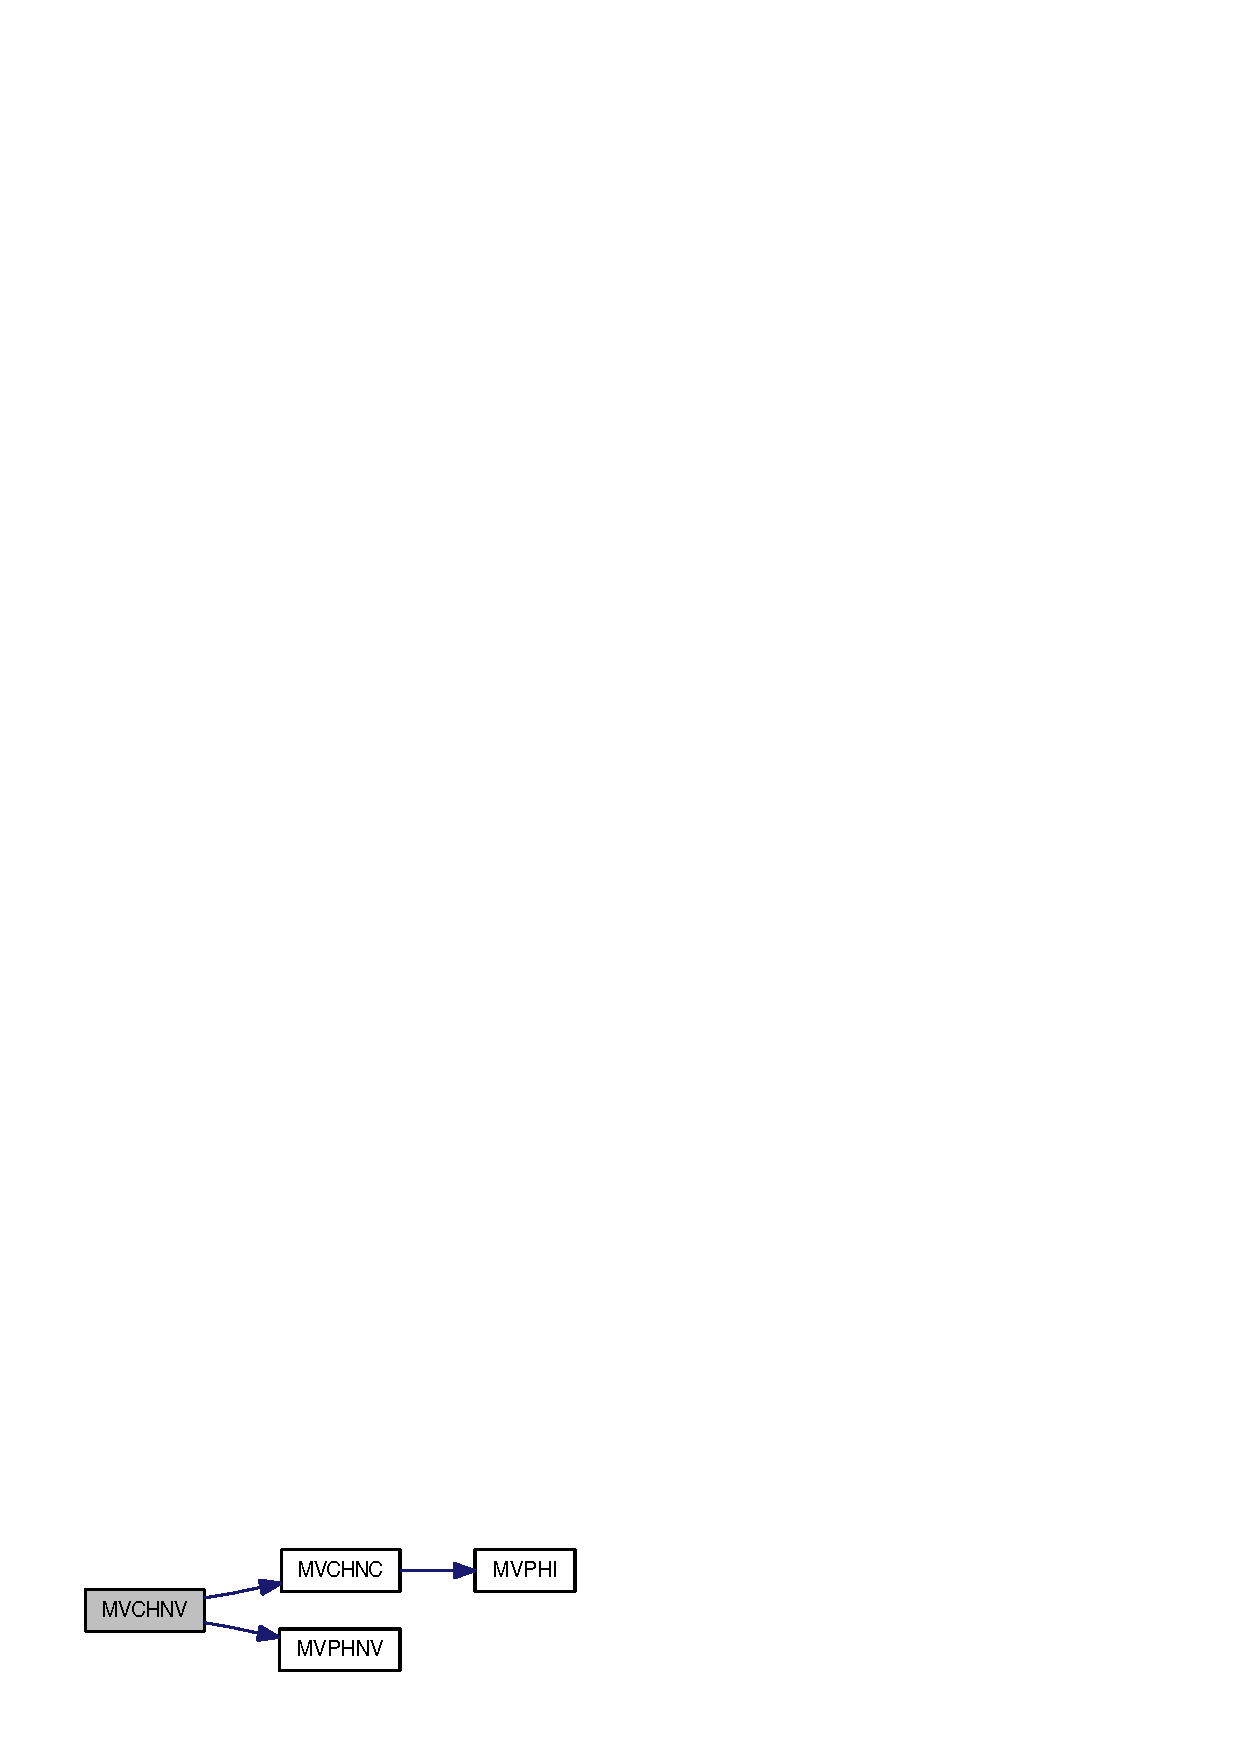
\includegraphics[width=140pt]{mvt_8f_3652f2cb737bf864d78fff1a650ca287_cgraph}
\end{center}
\end{figure}
\hypertarget{mvt_8f_53a2e447659c04eb0ad551cf58c77d37}{
\index{mvt.f@{mvt.f}!MVKBRV@{MVKBRV}}
\index{MVKBRV@{MVKBRV}!mvt.f@{mvt.f}}
\subsubsection[{MVKBRV}]{\setlength{\rightskip}{0pt plus 5cm}subroutine MVKBRV (INTEGER {\em NDIM}, \/  INTEGER {\em MINVLS}, \/  INTEGER {\em MAXVLS}, \/  INTEGER {\em NF}, \/  FUNSUB, \/  DOUBLE PRECISION {\em ABSEPS}, \/  DOUBLE PRECISION {\em RELEPS}, \/  DOUBLE PRECISION {\em ABSERR}, \/  DOUBLE PRECISION,dimension($\ast$) {\em FINEST}, \/  INTEGER {\em INFORM})}}
\label{mvt_8f_53a2e447659c04eb0ad551cf58c77d37}




Definition at line 1170 of file mvt.f.

References MVKRSV().

Referenced by MVTDST().

Here is the call graph for this function:\nopagebreak
\begin{figure}[H]
\begin{center}
\leavevmode
\includegraphics[width=181pt]{mvt_8f_53a2e447659c04eb0ad551cf58c77d37_cgraph}
\end{center}
\end{figure}
\hypertarget{mvt_8f_6b32b1cb4d3243c9ffef2622d8cfa65d}{
\index{mvt.f@{mvt.f}!MVKRSV@{MVKRSV}}
\index{MVKRSV@{MVKRSV}!mvt.f@{mvt.f}}
\subsubsection[{MVKRSV}]{\setlength{\rightskip}{0pt plus 5cm}subroutine MVKRSV (INTEGER {\em NDIM}, \/  INTEGER {\em KL}, \/  DOUBLE PRECISION,dimension($\ast$) {\em VALUES}, \/  INTEGER {\em PRIME}, \/  DOUBLE PRECISION,dimension($\ast$) {\em VK}, \/  INTEGER {\em NF}, \/  FUNSUB, \/  DOUBLE PRECISION,dimension($\ast$) {\em X}, \/  DOUBLE PRECISION,dimension($\ast$) {\em R}, \/  INTEGER,dimension($\ast$) {\em PR}, \/  DOUBLE PRECISION,dimension($\ast$) {\em FS})}}
\label{mvt_8f_6b32b1cb4d3243c9ffef2622d8cfa65d}




Definition at line 1443 of file mvt.f.

References MVUNI().

Referenced by MVKBRV().

Here is the call graph for this function:\nopagebreak
\begin{figure}[H]
\begin{center}
\leavevmode
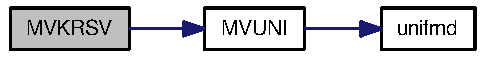
\includegraphics[width=134pt]{mvt_8f_6b32b1cb4d3243c9ffef2622d8cfa65d_cgraph}
\end{center}
\end{figure}
\hypertarget{mvt_8f_ae28c99f4b4ff2300cfa96ffa62bf799}{
\index{mvt.f@{mvt.f}!MVLIMS@{MVLIMS}}
\index{MVLIMS@{MVLIMS}!mvt.f@{mvt.f}}
\subsubsection[{MVLIMS}]{\setlength{\rightskip}{0pt plus 5cm}subroutine MVLIMS (DOUBLE PRECISION {\em A}, \/  DOUBLE PRECISION {\em B}, \/  INTEGER {\em INFIN}, \/  DOUBLE PRECISION {\em LOWER}, \/  DOUBLE PRECISION {\em UPPER})}}
\label{mvt_8f_ae28c99f4b4ff2300cfa96ffa62bf799}




Definition at line 451 of file mvt.f.

References MVPHI().

Referenced by MVSORT(), and MVVLSB().

Here is the call graph for this function:\nopagebreak
\begin{figure}[H]
\begin{center}
\leavevmode
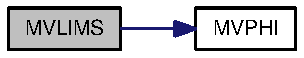
\includegraphics[width=91pt]{mvt_8f_ae28c99f4b4ff2300cfa96ffa62bf799_cgraph}
\end{center}
\end{figure}
\hypertarget{mvt_8f_a0072dd6ba4c47d28d78d231b5af9571}{
\index{mvt.f@{mvt.f}!MVPHI@{MVPHI}}
\index{MVPHI@{MVPHI}!mvt.f@{mvt.f}}
\subsubsection[{MVPHI}]{\setlength{\rightskip}{0pt plus 5cm}DOUBLE PRECISION MVPHI (DOUBLE PRECISION {\em Z})}}
\label{mvt_8f_a0072dd6ba4c47d28d78d231b5af9571}




Definition at line 500 of file mvt.f.

Referenced by MVBVU(), MVCHNC(), MVLIMS(), and MVSTDT().\hypertarget{mvt_8f_9ce2ff2aa4833561178c981ac2469470}{
\index{mvt.f@{mvt.f}!MVPHNV@{MVPHNV}}
\index{MVPHNV@{MVPHNV}!mvt.f@{mvt.f}}
\subsubsection[{MVPHNV}]{\setlength{\rightskip}{0pt plus 5cm}DOUBLE PRECISION MVPHNV (P)}}
\label{mvt_8f_9ce2ff2aa4833561178c981ac2469470}




Definition at line 550 of file mvt.f.

Referenced by MVCHNV(), and MVVLSB().\hypertarget{mvt_8f_e6a30b16d74f1c585c70de45080c0805}{
\index{mvt.f@{mvt.f}!MVSORT@{MVSORT}}
\index{MVSORT@{MVSORT}!mvt.f@{mvt.f}}
\subsubsection[{MVSORT}]{\setlength{\rightskip}{0pt plus 5cm}subroutine MVSORT (INTEGER {\em N}, \/  DOUBLE PRECISION,dimension($\ast$) {\em LOWER}, \/  DOUBLE PRECISION,dimension($\ast$) {\em UPPER}, \/  DOUBLE PRECISION,dimension($\ast$) {\em DELTA}, \/  DOUBLE PRECISION,dimension($\ast$) {\em CORREL}, \/  INTEGER,dimension($\ast$) {\em INFIN}, \/  DOUBLE PRECISION,dimension($\ast$) {\em Y}, \/  LOGICAL {\em PIVOT}, \/  INTEGER {\em ND}, \/  DOUBLE PRECISION,dimension($\ast$) {\em A}, \/  DOUBLE PRECISION,dimension($\ast$) {\em B}, \/  DOUBLE PRECISION,dimension($\ast$) {\em DL}, \/  DOUBLE PRECISION,dimension($\ast$) {\em COV}, \/  INTEGER,dimension($\ast$) {\em INFI}, \/  INTEGER {\em INFORM})}}
\label{mvt_8f_e6a30b16d74f1c585c70de45080c0805}




Definition at line 246 of file mvt.f.

References MVLIMS(), MVSSWP(), MVSWAP(), and MVTDNS().

Referenced by MVSUBR().

Here is the call graph for this function:\nopagebreak
\begin{figure}[H]
\begin{center}
\leavevmode
\includegraphics[width=147pt]{mvt_8f_e6a30b16d74f1c585c70de45080c0805_cgraph}
\end{center}
\end{figure}
\hypertarget{mvt_8f_cb964c59585b62348fb9653f052c669e}{
\index{mvt.f@{mvt.f}!MVSPCL@{MVSPCL}}
\index{MVSPCL@{MVSPCL}!mvt.f@{mvt.f}}
\subsubsection[{MVSPCL}]{\setlength{\rightskip}{0pt plus 5cm}subroutine MVSPCL (INTEGER {\em ND}, \/  INTEGER {\em NU}, \/  DOUBLE PRECISION,dimension($\ast$) {\em A}, \/  DOUBLE PRECISION,dimension($\ast$) {\em B}, \/  DOUBLE PRECISION,dimension($\ast$) {\em DL}, \/  DOUBLE PRECISION,dimension($\ast$) {\em COV}, \/  INTEGER,dimension($\ast$) {\em INFI}, \/  DOUBLE PRECISION {\em SNU}, \/  DOUBLE PRECISION {\em VL}, \/  DOUBLE PRECISION {\em ER}, \/  INTEGER {\em INFORM})}}
\label{mvt_8f_cb964c59585b62348fb9653f052c669e}




Definition at line 117 of file mvt.f.

References MVBVT(), and MVSTDT().

Referenced by MVSUBR().

Here is the call graph for this function:\nopagebreak
\begin{figure}[H]
\begin{center}
\leavevmode
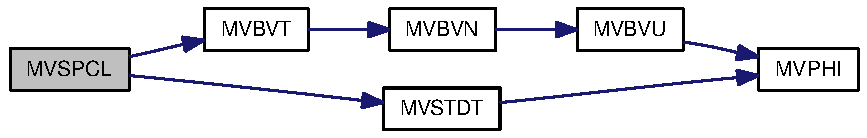
\includegraphics[width=226pt]{mvt_8f_cb964c59585b62348fb9653f052c669e_cgraph}
\end{center}
\end{figure}
\hypertarget{mvt_8f_2a36c253875e26e22bbb20a386c9a580}{
\index{mvt.f@{mvt.f}!MVSSWP@{MVSSWP}}
\index{MVSSWP@{MVSSWP}!mvt.f@{mvt.f}}
\subsubsection[{MVSSWP}]{\setlength{\rightskip}{0pt plus 5cm}subroutine MVSSWP (DOUBLE PRECISION {\em X}, \/  DOUBLE PRECISION {\em Y})}}
\label{mvt_8f_2a36c253875e26e22bbb20a386c9a580}




Definition at line 463 of file mvt.f.

Referenced by MVSORT(), and MVSWAP().\hypertarget{mvt_8f_33d5a1ab44132a99ec34a2a0c899cdcb}{
\index{mvt.f@{mvt.f}!MVSTDT@{MVSTDT}}
\index{MVSTDT@{MVSTDT}!mvt.f@{mvt.f}}
\subsubsection[{MVSTDT}]{\setlength{\rightskip}{0pt plus 5cm}DOUBLE PRECISION MVSTDT (INTEGER {\em NU}, \/  DOUBLE PRECISION {\em T})}}
\label{mvt_8f_33d5a1ab44132a99ec34a2a0c899cdcb}




Definition at line 822 of file mvt.f.

References MVPHI().

Referenced by MVSPCL().

Here is the call graph for this function:\nopagebreak
\begin{figure}[H]
\begin{center}
\leavevmode
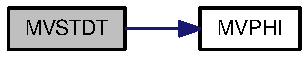
\includegraphics[width=92pt]{mvt_8f_33d5a1ab44132a99ec34a2a0c899cdcb_cgraph}
\end{center}
\end{figure}
\hypertarget{mvt_8f_1e3a3eb63d17fe37f686fc1f571beccc}{
\index{mvt.f@{mvt.f}!MVSUBR@{MVSUBR}}
\index{MVSUBR@{MVSUBR}!mvt.f@{mvt.f}}
\subsubsection[{MVSUBR}]{\setlength{\rightskip}{0pt plus 5cm}subroutine MVSUBR (INTEGER {\em N}, \/  DOUBLE PRECISION,dimension($\ast$) {\em W}, \/  INTEGER {\em NF}, \/  DOUBLE PRECISION,dimension($\ast$) {\em F})}}
\label{mvt_8f_1e3a3eb63d17fe37f686fc1f571beccc}




Definition at line 84 of file mvt.f.

References MVCHNV(), MVSORT(), MVSPCL(), and MVVLSB().

Referenced by MVTDST().

Here is the call graph for this function:\nopagebreak
\begin{figure}[H]
\begin{center}
\leavevmode
\includegraphics[width=283pt]{mvt_8f_1e3a3eb63d17fe37f686fc1f571beccc_cgraph}
\end{center}
\end{figure}
\hypertarget{mvt_8f_5411cfeafe20ca2bd17c962f8c8c0e84}{
\index{mvt.f@{mvt.f}!MVSWAP@{MVSWAP}}
\index{MVSWAP@{MVSWAP}!mvt.f@{mvt.f}}
\subsubsection[{MVSWAP}]{\setlength{\rightskip}{0pt plus 5cm}subroutine MVSWAP (INTEGER {\em P}, \/  INTEGER {\em Q}, \/  DOUBLE PRECISION,dimension($\ast$) {\em A}, \/  DOUBLE PRECISION,dimension($\ast$) {\em B}, \/  DOUBLE PRECISION,dimension($\ast$) {\em D}, \/  INTEGER,dimension($\ast$) {\em INFIN}, \/  INTEGER {\em N}, \/  DOUBLE PRECISION,dimension($\ast$) {\em C})}}
\label{mvt_8f_5411cfeafe20ca2bd17c962f8c8c0e84}




Definition at line 470 of file mvt.f.

References MVSSWP().

Referenced by MVSORT().

Here is the call graph for this function:\nopagebreak
\begin{figure}[H]
\begin{center}
\leavevmode
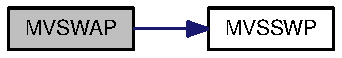
\includegraphics[width=100pt]{mvt_8f_5411cfeafe20ca2bd17c962f8c8c0e84_cgraph}
\end{center}
\end{figure}
\hypertarget{mvt_8f_7edd239860c89b5fa9fb100b194fa833}{
\index{mvt.f@{mvt.f}!MVTDNS@{MVTDNS}}
\index{MVTDNS@{MVTDNS}!mvt.f@{mvt.f}}
\subsubsection[{MVTDNS}]{\setlength{\rightskip}{0pt plus 5cm}DOUBLE PRECISION MVTDNS (INTEGER {\em NU}, \/  DOUBLE PRECISION {\em X})}}
\label{mvt_8f_7edd239860c89b5fa9fb100b194fa833}




Definition at line 429 of file mvt.f.

Referenced by MVSORT().\hypertarget{mvt_8f_4b51e2fd2b5378c70a36771ac4cfed04}{
\index{mvt.f@{mvt.f}!MVTDST@{MVTDST}}
\index{MVTDST@{MVTDST}!mvt.f@{mvt.f}}
\subsubsection[{MVTDST}]{\setlength{\rightskip}{0pt plus 5cm}subroutine MVTDST (INTEGER {\em N}, \/  INTEGER {\em NU}, \/  DOUBLE PRECISION,dimension($\ast$) {\em LOWER}, \/  DOUBLE PRECISION,dimension($\ast$) {\em UPPER}, \/  INTEGER,dimension($\ast$) {\em INFIN}, \/  DOUBLE PRECISION,dimension($\ast$) {\em CORREL}, \/  DOUBLE PRECISION,dimension($\ast$) {\em DELTA}, \/  INTEGER {\em MAXPTS}, \/  DOUBLE PRECISION {\em ABSEPS}, \/  DOUBLE PRECISION {\em RELEPS}, \/  DOUBLE PRECISION {\em ERROR}, \/  DOUBLE PRECISION {\em VALUE}, \/  INTEGER {\em INFORM})}}
\label{mvt_8f_4b51e2fd2b5378c70a36771ac4cfed04}




Definition at line 4 of file mvt.f.

References MVKBRV(), and MVSUBR().

Here is the call graph for this function:\nopagebreak
\begin{figure}[H]
\begin{center}
\leavevmode
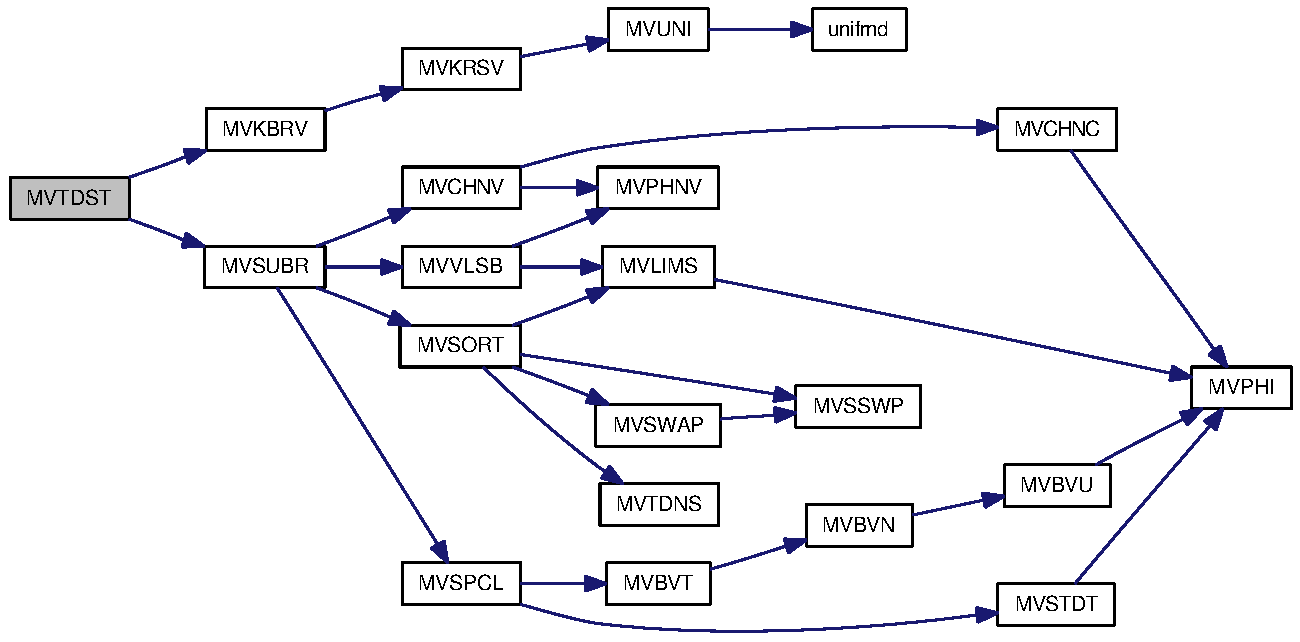
\includegraphics[width=330pt]{mvt_8f_4b51e2fd2b5378c70a36771ac4cfed04_cgraph}
\end{center}
\end{figure}
\hypertarget{mvt_8f_1ab822a6524a9096bf2ec00253f890e3}{
\index{mvt.f@{mvt.f}!MVUNI@{MVUNI}}
\index{MVUNI@{MVUNI}!mvt.f@{mvt.f}}
\subsubsection[{MVUNI}]{\setlength{\rightskip}{0pt plus 5cm}DOUBLE PRECISION MVUNI ()}}
\label{mvt_8f_1ab822a6524a9096bf2ec00253f890e3}




Definition at line 1489 of file mvt.f.

References unifrnd().

Referenced by MVKRSV().

Here is the call graph for this function:\nopagebreak
\begin{figure}[H]
\begin{center}
\leavevmode
\includegraphics[width=87pt]{mvt_8f_1ab822a6524a9096bf2ec00253f890e3_cgraph}
\end{center}
\end{figure}
\hypertarget{mvt_8f_7319671edcfbb7bd0e50690518e644fc}{
\index{mvt.f@{mvt.f}!MVVLSB@{MVVLSB}}
\index{MVVLSB@{MVVLSB}!mvt.f@{mvt.f}}
\subsubsection[{MVVLSB}]{\setlength{\rightskip}{0pt plus 5cm}subroutine MVVLSB (INTEGER {\em N}, \/  DOUBLE PRECISION,dimension($\ast$) {\em W}, \/  DOUBLE PRECISION {\em R}, \/  DOUBLE PRECISION,dimension($\ast$) {\em DL}, \/  INTEGER,dimension($\ast$) {\em INFI}, \/  DOUBLE PRECISION,dimension($\ast$) {\em A}, \/  DOUBLE PRECISION,dimension($\ast$) {\em B}, \/  DOUBLE PRECISION,dimension($\ast$) {\em COV}, \/  DOUBLE PRECISION,dimension($\ast$) {\em Y}, \/  DOUBLE PRECISION {\em DI}, \/  DOUBLE PRECISION {\em EI}, \/  INTEGER {\em ND}, \/  DOUBLE PRECISION {\em VALUE})}}
\label{mvt_8f_7319671edcfbb7bd0e50690518e644fc}




Definition at line 194 of file mvt.f.

References MVLIMS(), and MVPHNV().

Referenced by MVSUBR().

Here is the call graph for this function:\nopagebreak
\begin{figure}[H]
\begin{center}
\leavevmode
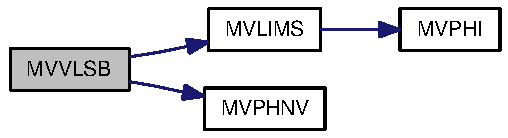
\includegraphics[width=140pt]{mvt_8f_7319671edcfbb7bd0e50690518e644fc_cgraph}
\end{center}
\end{figure}
